\section{Estratégia de Recuperação de Sessões Pós-Quânticas}
\label{sec:proposta}

A estratégia avaliada combina checkpoints autenticados, estabelecimento de chaves de tráfego novas e registro das decisões da aplicação antes da confirmação. O cliente estabelece a conexão por retomada ou autenticação completa, enquanto o gateway reconhece leituras já processadas. A implementação permite comparar políticas de preservação do contexto de retomada e configurações criptográficas, relacionando as falhas ao custo da recuperação por leitura confirmada.

\subsection{Modelagem do Problema}
\label{sec:modelagem}

Considera-se um sensor \(d\), um gateway \(g\) e uma leitura \(r=(d,u,m)\), em que \(u\) é o identificador preservado entre tentativas e \(m\) é o conteúdo. A sessão salva no cliente permite oferecer uma retomada; o contexto do gateway determina sua aceitação; e o banco conserva os registros das leituras processadas. Esses três estados permitem distinguir as consequências de sua perda ou restauração.

O primeiro desafio é a não reutilização da combinação de chave e nonce, conforme a Equação~\ref{eq:unicidade_nonce}. O protótipo compara a restauração de chaves e contadores, incluindo seus registros salvos, com modos que estabelecem chaves novas. No TLS nativo, o checkpoint fornece o contexto de retomada; a biblioteca negocia outra conexão e deriva suas chaves com contribuição assimétrica nova.

O segundo desafio é a disponibilidade do contexto no gateway. O TLS utiliza tickets que transportam estado protegido, sem cache por sessão. Na política com contexto perdido, a chave de proteção dos tickets é substituída a cada reinício; na política com contexto preservado, a mesma chave é carregada novamente. Ambas utilizam a mesma construção de tickets e conservam o banco de leituras. Um terceiro modo realiza autenticação completa diretamente em cada tentativa, servindo como comparador.

O terceiro desafio é reconhecer uma leitura processada cuja confirmação se perdeu. O banco associa \((d,u)\) ao SHA-256 do conteúdo e aplica a decisão da Equação~\ref{eq:decisao_leitura}: registrar uma leitura nova, confirmar uma repetição correspondente ou rejeitar conteúdo conflitante para o mesmo identificador.

O modelo considera reinícios, rollback e interrupções da comunicação. No protótipo, cada falha é seguida de nova tentativa sem interrupção. Nos estudos de caso TLS, variam-se as frequências de reinício do gateway e de supressão da confirmação, que podem coincidir na mesma leitura. A supressão encerra a conexão após a gravação no banco e antes da resposta, diferindo da perda de um pacote TCP recuperável pelo transporte.

Credenciais de identidade, chave de proteção do checkpoint e fontes de entropia ficam fora do rollback do cliente. A restauração de todo o banco do gateway é avaliada em um controle separado, que elimina registros necessários à deduplicação. Esse controle não integra a comparação das políticas de preservação da chave dos tickets.

Os critérios distinguem a não reutilização da combinação de chave e nonce, a autenticação e a repetição de efeitos. O protótipo observa os pares utilizados na cifragem; o TLS verifica identidades, parâmetros e compartilhamentos públicos novos, sem exportar chaves de tráfego ou vetores de inicialização. O efeito avaliado é uma inserção no banco do gateway.

A Figura~\ref{fig:propostafig} sintetiza a estratégia para tratar esses desafios. O fluxo verifica o checkpoint, estabelece uma conexão com chaves novas e consulta o banco antes da confirmação. Quando a confirmação se perde, o controlador repete a leitura com o mesmo identificador, denominado código na figura, respeitando o limite de tentativas. Leituras repetidas são reconhecidas sem reaplicar o efeito quando a deduplicação está ativa.

\begin{figure}[!htb]
\centering
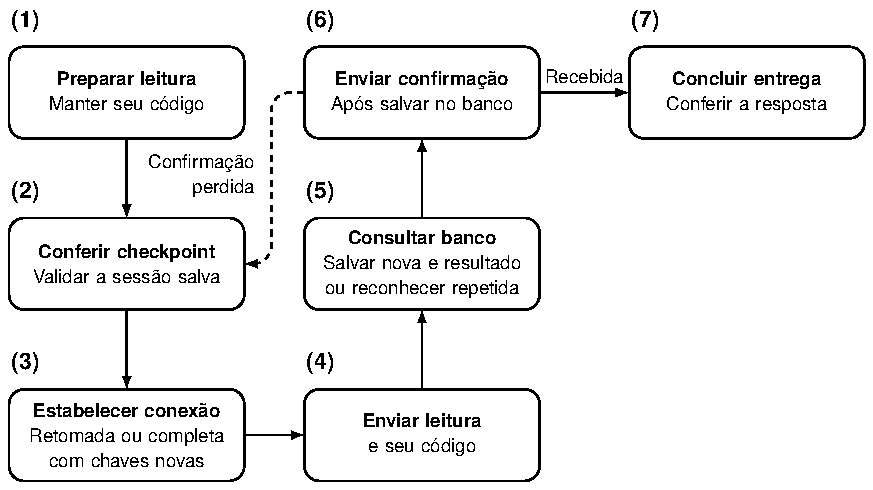
\includegraphics[width=0.95\linewidth]{figuras/figura_3_recuperacao_sessoes.pdf}
\caption{Estratégia de recuperação de sessões e confirmação de leituras. O reenvio conserva a leitura e seu código.}
\label{fig:propostafig}
\end{figure}

\subsection{Estratégia de Recuperação e Confirmação de Leituras}

Nas etapas (1) e (2), o controlador prepara a leitura e conserva seu identificador entre tentativas. O cliente inicia um processo novo, carrega as credenciais e verifica o checkpoint. A sessão salva é protegida por AES-GCM e vinculada ao nome do servidor e à autoridade certificadora (CA) esperados. O arquivo anterior só é substituído após a gravação completa da nova cópia, evitando um arquivo parcialmente gravado. A atualização é sincronizada com o armazenamento para permanecer disponível após reinícios. Arquivo ausente, conteúdo adulterado ou vínculo incompatível impede a oferta da sessão e leva ao handshake completo. Uma cópia antiga e autêntica pode continuar válida, dependendo do contexto do gateway.

As conexões utilizam TLS 1.3, autenticação mútua e AES-256-GCM com SHA-384. A configuração clássica combina X25519 e ECDSA P-256; a híbrida utiliza X25519MLKEM768 e ECDSA P-256; e a pós-quântica combina X25519MLKEM768 e ML-DSA-44. Aplicação, carga e cenários são mantidos entre os comparadores. A retomada acrescenta uma contribuição assimétrica nova ao segredo anterior, e erros de identidade encerram a tentativa. O envio antecipado de dados, denominado 0-RTT, permanece desabilitado.

Na etapa (3), o cliente apresenta a sessão salva quando ela está disponível nas políticas de retomada. Se o gateway não consegue recuperar o estado do ticket, a negociação prossegue com autenticação completa na mesma conexão, mantendo a configuração criptográfica. O OpenSSL executa o protocolo e a derivação de chaves. Quando uma sessão retomável fica disponível após o processamento dos tickets, o cliente a salva. A instrumentação distingue a retomada aceita da autenticação completa após uma oferta recusada.

Nas etapas (4) e (5), o cliente envia identificador e conteúdo pela conexão autenticada. O gateway consulta o banco e aplica o efeito apenas para uma leitura nova quando a deduplicação está ativa. Repetições correspondentes são confirmadas sem reaplicar o efeito; conflitos são rejeitados. O registro da leitura e o efeito são gravados juntos em uma única operação no SQLite, de modo que ambos sejam salvos ou nenhum deles seja. A gravação termina antes da confirmação, e os registros permanecem disponíveis após reinícios.

Nas etapas (6) e (7), o gateway envia a confirmação com o identificador, o resumo do conteúdo e o reconhecimento de repetição. O cliente confere a resposta antes de concluir a entrega. Se a confirmação se perde, o controlador retorna à etapa (2), iniciando outro processo com a mesma leitura e o mesmo identificador. O reenvio não sofre outra interrupção lógica programada e respeita o limite de três tentativas por leitura. A ausência de confirmação após esse limite é registrada como entrega não concluída. O banco permite reconhecer o processamento anterior mesmo quando a nova tentativa utiliza outra sessão.

Nos experimentos, o controlador mantém os dados pendentes entre processos; uma fila persistente no armazenamento do sensor permanece como extensão da implementação. O controle experimental desativa somente a supressão dos efeitos repetidos, mantendo o rastreamento dos identificadores e a rejeição de conflitos.

Por fim, registram-se bytes, tempos, parâmetros e decisões sobre as leituras. Os custos seguem a Equação~\ref{eq:custo_recuperacao}, incluindo ofertas de retomada recusadas, novas tentativas e encerramentos das conexões. O tempo até a confirmação considera também a inicialização do gateway quando prevista. A análise relaciona esses custos às configurações criptográficas, às políticas de estado e às frequências de falhas, mantendo separados os efeitos registrados no banco.
